\chapter{Crittografia Asimmetrica e Scambio di Chiavi}

\section{Diffie-Hellman}
Per ovviare al problema dei cifrari simmetrici per quanto riguarda la \textit{gestione delle chiavi} nel 1976 viene pubblicato un articolo \textit{``New Direction in Cryptography''}, pubblicato da due ricercatori: Whitfield Diffie e Martin Hellman. La loro intuizione fu quella di poter utilizzare nella cifrazione e nella corrispondente decifratura due chiavi differenti. Se si potesse allora si potrebbe \textbf{condividere} la \textbf{chiave di cifratura} e quindi utilizzabile da chiunque mentre la \textbf{chiave di decifrazione} tenuta \textbf{privata}. Lo schema introduce il ``problema'' della gestione delle chiavi pubbliche che però non è totalmente risolvibile a livello algoritmico.
\newline
Il \textbf{protocollo} introdotto da \textit{DH} non è uno schema a chiave pubblica, ma un metodo per la \textbf{comunicazione di informazione segreta su un canale di comunicazione insicuro}. Questo protocollo viene tutt'ora utilizzato all'interno di molti altri protocolli di sicurezza su internet, tra cui: \textit{TLS} e \textit{SSH}.
\\ \newline
\textbf{Il protocollo DH su gruppi ciclici $\mathbb{Z}_p^*$}
\newline
In questo protocolo \textit{Alice} e \textit{Bob} utilizzano un \textbf{protocollo simmetrico} per comunicare, per farlo bisogna che però si scambino una chiave condivisa da tenere segreta tramite un canale insicuro. Il protocollo di Diffie e Hellman consente alle due parti di concordare un segreto che altro non è che un elemento di un oppportuno gruppo $\mathbb{Z}_p^*$. Utilizzando tale segreto, le due parti \textbf{deriveranno la chiave} da usare nel protocollo.
\\ \newline
\textbf{Algoritmo DH}
\begin{enumerate}
    \item \textit{Alice} e \textit{Bob} si accordano sul \textbf{modulo p} da utilizzare, deve essere un numero primo, e sull'uso di una \textbf{radice primitiva} $g \in \mathbb{Z}_p^*$.
    \begin{itemize}
        \item tutto questo viene fatto \textbf{pubblicamente} e quindi anche un malvivente \textit{Eve} li conosce.
        \item \textit{p} e \textit{g} vengono scelta da chi inizia la comunicazione e confermati dall'altra parte.
    \end{itemize}
    \item \textit{Alice} sceglie con \textbf{distribuzione di probabilità uniforme} un numero $a \in \mathbb{Z}_p^*$, con il quale calcola $x_a = g^a \bmod p$ e invia $x_a$ a \textit{Bob}.
    \item in modo simile \textit{Bob} sceglie un elemento $b \in \mathbb{Z}_p^*$ e con questo valore calcola $x_b = g^b \bmod p$ e invia $x_b$ ad \textit{Alice}.
    \item con l'informazione $x_a$ inviata da \textit{Alice}, \textit{Bob} si calcola il valore $z_a = x_a^b \bmod p$.
    \item analogamente \textit{Alice} si calcola il valore $z_b = x_b^a \bmod p$ con il valore $x_b$ inviato da \textit{Bob}.
    \item la quantità $z = z_a = z_b$ è il \textbf{segreto condiviso}.
\end{enumerate}
È possibile verificare l'ugualianza $z_a = z_b$:
\begin{center}
    \begin{math}
        \begin{aligned}
            z_a &= x_b^a \bmod p \\
            &= (g^b \bmod p)^a \bmod p \\
            &= (g^b)^a \bmod p \\
            &= (g^a)^b \bmod p \\
            &= (g^a \bmod p)^b \bmod p \\
            &= x_a^b \bmod p \\
            &= z_b
        \end{aligned}
    \end{math}
\end{center}
L'\textbf{Efficenza} del protocollo è dovuto al fatto che tutte le quantità necessarie sono facilemnte calcolabili in maniera efficente, le computazioni più onerose sono i due esponenziali modulari che hanno \textbf{complessità polinomiale} sulla base della lunghezza dei valori (in bit). La vera computazione è nella ricerca di un primo ``adatto'', infatti bisogna trovare un \textit{p} primo che abbia come \textbf{generatore} un valore \textit{g} che abbia ordine $ord(g) = p - 1$. La ricerca di un primo ``adatto'' avviene tramite un \textbf{\textit{safe prime}} con generatore \textbf{``fisso''}.
\\
La \textbf{Sicurezza} si basa sulla difficoltà algoritmica da parte di \textit{Eve} di calcolare \textit{z} dalle informazioni girate in maniera insicura ovvero: il primo \textit{p} il generatore \textit{g} e le due chiavi pubbliche $x_a$ e $x_b$. \textit{Eve} può effettuare tutte le operazioni che vuole su $\mathbb{Z}_p^*$ ma \textit{Eve} necessiterebbe di una delle due chiavi private o \textit{a} o di \textit{b} e questo richiederebbe il calcolo del \textbf{logaritmo discreto} per invertire $x_a$ e $x_b$ infatti $x_a = \log_{g}{x_a} \bmod p$. Ovviamente la situazione è la stessa se \textit{Eve} vuole reversare la \textit{chiave segreta z}.
\\ \newline
\textbf{\textit{Computational Diffie-Hellman Assumptions}} se \textit{g}, \textit{a} e \textit{b} sono scelti a caso in $\mathbb{Z}_p^*$ allora, a partire da \textit{g}, $g^a \bmod p$ e $g^b \bmod p$ la determinazione di $g^{ab} \bmod p$ è un problema \textbf{computazione intrattabile}. \\
Il dato condiviso da \textit{Alice} e \textit{Bob} non è generalmente utilizzabile come chiave segreta in un protocollo di crittografia simmetrica, infatti le chiavi che cerchiamo sono stringhe di bit che hanno, per singolo bit, la stessa probabilità di essere o \textit{0} o \textit{1}. Nel nostro caso il segreto condiviso invece è un numero uniformemente distribuito in $\mathbb{Z}_p^*$ che ovviamente non è la stessa cosa. Infatti in un caso di $\mathbb{Z}_{11}^*$ avremo che la possibilità del bit di essere \textit{1} in posizione $2^2$ sarà lo $0.2\%$ a differenza dei bit in posizione $2^0$ e $2^1$ che invece avranno probabilità di essere \textit{1} pari a quella di essere \textit{0} ovvero $0.5\%$. Questo devia molto dalla situazione ideale che vorremmo ottenere per una chiave privata in un protocollo simmetrico. Per riuscire ad estrarre \textbf{entropia} dal segreto viene applicato al segreto condiviso una funzione \textbf{hash crittografica} (identica tra \textit{Alice} e \textit{Bob}) il cui output viene usato come chiave simmetrica.
\\ \newline
\textbf{Attacchi a DH}: visto la \textit{computational diffie-hellman assumptions} attacchi diretti per determinare $g^{ab} \bmod p$ sono \textbf{computazionalmente infattibili}. Un attacco vincente è invece il \textbf{Man-in-the-Middle}. Nel caso in cui \textit{Eve} si interponga tra \textit{Alice} e \textit{Bob} e si riesca a fingere \textit{Alice} rispetto a \textit{Bob} e viceversa, potrà partecipare ad un doppio scambio di chiavi, questo è possibile in quanto \textit{diffie-hellman} non fornisce un protocollo sicuro di autenticazione. A seconda degli obiettivi, \textit{Eve}, potrà modificiare i messaggi (attacco a \textbf{breve termine}) o lasciarli inalterati (attacco a \textbf{lungo termine}). 
\\ \newline
\textbf{\textit{Authenticated Diffie-Hellman}}
\newline
È chiaro che qual'ora \textit{Alice} e \textit{Bob} riuscissero ad \textbf{autenticarsi} l'uno rispetto all'altro e viceversa, un attacco \textbf{man-in-the-middle} sarebbe irrealistico in quanto, prendendolo come esempio, \textit{Alice} riuscirebbe a svelare l'impersonificazione di \textit{Eve}. Per poter riuscire ad autenticarsi è quindi necessario ricorrere alla \textbf{firma digitale}, ovvero entrambi le parti deve possedere anticipatamente una chiave pubblica. 
\begin{center}
    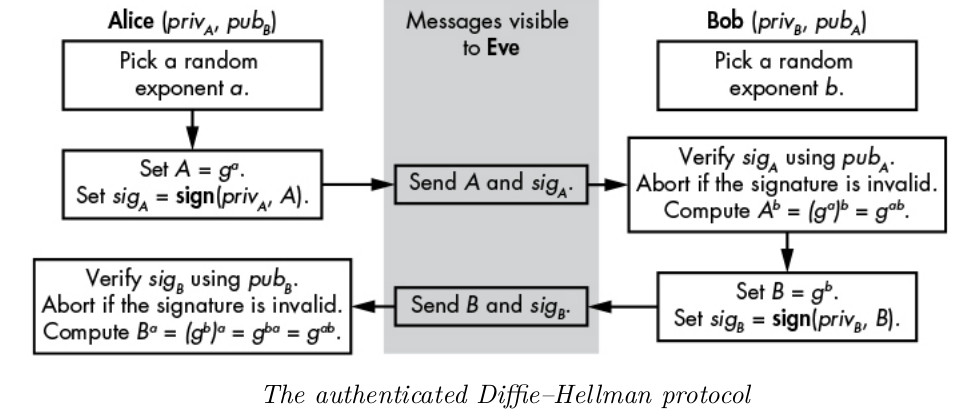
\includegraphics[width=0.8\textwidth]{authDH.jpg}
\end{center}
In generale in un protocollo per lo scambio sicuro di chiavi, c'è la necessità che almeno una delle due parti disponga di un \textbf{long-term secret} come può essere uno chiave \textbf{RSA}, ma a questo punto perché non usare direttamente una crittografia asimmetrica invece che un protocollo di scambio chiavi. Questo tipo di approccio \textbf{non} garantisce \textbf{\textit{forward-secrecy}}. \\
La \textbf{\textit{Forward Secrecy}} è una proprietà dei protocolli di \textit{negoziazione delle chiavi} che assicura che se una chiave di cifratura a lungo termine (\textit{long-term secret}) viene compromessa, le chiavi di sessione generate a partire da essa rimangono riservate. \\ \newline
\textbf{\textit{Ephemeral Diffie-Hellman Keys}} \\
In \textbf{\textit{TLS 1.3}} le chiavi simmetriche sono invece generatea partire da \textit{chiavi DH effimere}, questo implica che la chiave pubblica e privata dopo essere usate una sola volta, vengono \textbf{scartate da client e server}.

\newpage

\section{ElGamal}
Nel 1985 \textbf{\textit{ElGamal}} propone un sistema crittografico a chiave pubblica, questo viene pubblicato qualche anno dopo \textbf{RSA} (1977), ma lo affronteremo prima per una similitudine con \textit{Diffie-Hellman}. Poiché non venne brevettato, il sistema crittografico di \textit{ElGamal} venne inserito, insieme al protocollo \textbf{DSA} (\textit{Digital Signature Algorithm}), in molte suite crittografiche, tra tutte: \textbf{\textit{GNUPG}}. All'interno di \textit{ElGamal} possiamo identificare, come in qualunque altro algoritmo di crittografia asimmetrica due elementi:
\begin{enumerate}
    \item \textbf{generazione di una coppia di chiavi}, pubblica (che può essere resa disponibile) e privata.
    \item processo di comunicazione, composto a sua volta dalla \textbf{cifratura} e \textbf{decifratura}.
\end{enumerate}
\   \\
Per la parte di generazione della coppia di chiavi, inizialmente, \textit{Alice} determina i \textit{parametri} del protocollo:
\begin{itemize}
    \item un \textit{numero \textbf{p} primo} di lunghezza appropriata.
    \item una \textit{radice primitiva \textbf{g}} di $\mathbb{Z}_p^*$.
    \item calcolare il valore $A = g^a \bmod p$ dove $a \in \mathbb{Z}_p^*$ è un numero scelto uniformemente a caso.
\end{itemize}
Una volta determinati i paramentri \textit{Alice} conserverà \textit{a} come \textbf{chiave segreta} e provvederà a diffondere la terna \textit{(p, g, A)} come corrispondente \textbf{chiave pubblica}. Come possiamo notare, per questa prima parte del protocollo la differenza con \textit{DH} è solo nei destinatari della comunicazione, infatti non è più solo \textit{Bob} ma tutti. Nel momento in cui \textit{Bob} vuole inviare un messaggio cifrato ad \textit{Alice}, \textit{Bob} ottiene la chiave pubblica di \textit{Alice}, ovvero la terna \textit{(p, g, A)} e, dopo aver scelto un valore $b \in \mathbb{Z}_p^*$ uniformemente a caso, si calcola due quantità:
\begin{enumerate}
    \item $B = g^b \bmod p$
    \item $Cipher = (A^b * M) \bmod p$ dove M è il messaggio che \textit{Bob} vuole inviare ad \textit{Alice}.
\end{enumerate}
Inviando ad \textit{Alice} la coppia $C = (B, c)$ che costituisce il messaggio cifrato. Una volta ottenuto la coppia $(B, c)$ che costituisce il messaggio cifrato \textit{Alice} potrà decifrare il messaggio calcolando per prima cosa $Z = B^a \bmod p$ riuscendo ad ottenere attraverso l'uso del \textit{teorema di Euclide Esteso} il valore $Z^{-1} \bmod p$ e riuscendo a riottenere il messaggio in chiaro $M = (Z^{-1} * c) \bmod p$, si noti che il messaggio deve essere interpretabile come un numero \textbf{minore di p}. La \textbf{correttezza} dell'algoritmo è conseguenza del fatto che $Z = B^a \bmod p = A^b \bmod p$, ed è esattamente la stessa dimostrazione avvenuta per il teorema di \textit{diffie-hellman}.
\\ \newline
L'\textbf{Efficenza} è dovuta che la complessità della cifratura è dominata da due calcoli di potenze modulari, a cui va aggiunto il prodotto, mentre per il resto si tratta di pre-computazione delle chiavi. Al contrario la decifratura richiede il calcolo di una potenza, di un inverso e di una moltiplicazione. Un numero sostanzialmente molto ridotto di operazioni onerose che però bisogna considerare su numeri di oltre 1000 bit. Nel caso in cui il messaggio fosse più lungo della lunghezza del modulo \textit{p}, \textit{Bob} dovrebbe spezzare il messaggio in blocchi e ripetere la cifratura usando un valore di \textit{k} diverso per ogni singolo blocco. Con molti blocchi, e quindi con messaggi molto lunghi, cifratura e decifratura asimmetrica diventano dei passaggi molto onerosi soprattuto se confrontati con processi di cifratura simmetrica che oggigiorno supportano anche accelleratori hardware. Per questa ragione, la crittografia asimmetrica viene utilizzata in sinergia a quella simmetrica, in particolare, protocolli \textit{asimmetrici} vengono utilizzati in fase di \textit{autenticazione} delle parti e per lo \textit{scambio di chiavi}, mentre per la \textit{comunicazione} vera e propria viene utilizzato un protocollo \textit{simmetrico}. \\
Andando ad osservare invece la \textbf{Sicurezza} di \textit{ElGamal}, questa si basa sulla \textit{Computational Diffie-Hellman Assumptions} (\textbf{CDHA}) ovvero girando il problema che supponendo di riuscire a rompere \textit{ElGamal} e quindi di essere in grado di risolvere l'assunzione \textbf{\textit{CDH}}, infatti \textit{ElGamal} ``oscura'' il messaggio moltiplicando ($\times_p$) proprio per una quantità $A^b \bmod p$ che corrisponde al \textbf{segreto condiviso di DH}. Se dunque siamo in grado di decifrare \textit{M} (senza utilizzare il calcolo diretto del logaritmo discreto $a = \log_{g}{M} \bmod p$) allora possiamo risalire alla quantità $A^b \bmod p = g^{ab} \bmod p$ ovvero proprio la quantità che la \textbf{\textit{CDH Assumptions}} chiede di calcolare. Se quindi vale l'ipotesi \textit{CDHA} possiamo dedurre che \textbf{ElGamal è SICURO}. \\
Un errore da non commettere è di utilizzare per cifrature differenti lo stesso valore \textit{b}, infatti se questo dovesse valere, allora anche \textit{B} non cambia, quindi le cifrature di $M_1 \text{ e } M_2$ risulterebbero:
\begin{center}
    $C_1 = (B, c_1 = (A^b * M_1) \bmod p) \qquad \text{ e } \qquad C_2 = (B, c_2 = (A^b * M_2) \bmod p)$ \\
    Consideriamo ora $C_1$ \\\   \newline
    \begin{math}
        \begin{aligned}
            C_1 &= (B, c_2) \\
            &= (g^b \bmod p,\;A^b * M_1 \bmod p) \\
            &= (g^b \bmod p,\;g^{ab} * M_1 \bmod p) \\
            &= (g^b \bmod p,\;Z * M_1 \bmod p) \qquad Z = B^a \bmod p = g^{ab} \bmod p
        \end{aligned}
    \end{math}    
\end{center}
\begin{center}
    $c_2 = Z * M_2 \bmod p \qquad M_2 = Z^{-1} * M_2 \bmod p$ \\
    Moltiplichiamo a destra e a sinistra per $c_1^{-1}$ \\
    \begin{math}
        \begin{aligned}
            c_1^{-1} * c_2 \bmod p &= c_1^{-1} * (Z * M_2) \bmod p \\ 
            &= (A^b * M_1)^{-1} * (Z * M_2) \bmod p \\
            &= (g^{ab} * M_1)^{-1} * (Z * M_2) \bmod p \\
            &= (Z * M_1)^{-1} * (Z * M_2) \bmod p \\
            &= Z^{-1} * Z * (M_1^{-1} * M_2) \bmod p \\
            &= (M_1^{-1} * M_2) \bmod p \\
        \end{aligned}
    \end{math}
\end{center}
\begin{center}
    Moltiplichiamo a destra e a sinistra per $M_1$ \\
    \colorbox{yellow}{$M_2 = M_1 * (c_1^{-1} * c_2) \bmod p$}
\end{center}
Se \textit{Eve} fosse in grado (per qualsiasi motivo) di decifrare il messaggio $M_1$, e quindi avere la coppia $(M_1, \; c_1)$ potrebbe decifrare anche i successivi messaggi cifrati con lo stesso valore \textit{b}.

\newpage
\section{Sistema Crittografico RSA}
Il sistema crittografico \textbf{RSA} prende il nome dalle iniziali dei loro inventori: \textit{Ronald L. Rivest}, \textit{Adi Shamir} e \textit{Leonard M. Adlemam}. \textit{RSA} basa la sua efficacia, in termine di \textbf{sicurezza}, sulla difficoltà computazionale del \textbf{problema della fattorizzazione di numeri interi}, ovvero sul fatto che ad oggi non esistono algoritmi efficienti per fattorizzare numeri di grandi dimensioni. Ad oggi, però, non esiste un argomentazione matematica, come nel caso di \textit{Diffie-Hellman}, che dimostri che saper violare efficientemente RSA implichi saper fattorizzare numeri interi. \\
\textcolor{violet}{\textbf{\textit{Warning}}}: un \textbf{computer quantistico} sarebbe in grado di fattorizzare in maniera efficacie i numeri interi e quindi violare RSA.
\\ \newline
L'\textbf{Algoritmo in Dettaglio}: come in ogni cifrario asimmetrico la generazione delle chiavi è eseguita dal destinatario del ciphertext, che identificheremo come \textit{Alice}, il protocollo ha un solo parametro di input, che è la lunghezza in bit, indicata con \textit{N}, dell'intero con cui si effettuano le riduzioni modulari.
\begin{itemize}
    \item \textbf{Generazione delle Chiavi: \textit{Alice}}
    \begin{enumerate}
        \item generare due primi a casa \textit{p} e \textit{q} di lunghezza $\frac{N}{2}$.
        \item calcolare il prodotto $n = p * q$.
        \item calcolare $\phi(n) = (p - 1) * (q - 1)$.
        \item determinare un intero \textit{e}, (normalmente $e = 65537$) e relativamente primo con $\phi(n)$ ovvero che $gcd(e, \phi(n)) = 1$.
        \item calcolare l'inverso moltiplicativo \textit{d} di \textit{e} modulo $\phi(n)$, che esiste perché \textit{e} è \textbf{coprimo} con $\phi(n)$.
        \item diffondere la coppia (\textbf{\textit{e}}, \textbf{\textit{n}}) come \textbf{chiave pubblica} e conservare \textbf{\textit{b}} come \textbf{chiave privata}.
    \end{enumerate}
    \item \textbf{Cifratura del Messaggio M: \textit{Bob}}
    \begin{enumerate}
        \item si procura la chiave pubblica di \textit{Alice}, (\textbf{\textit{e}}, \textbf{\textit{n}}).
        \item calcola $C = M^e \bmod n$.
        \item invia \textit{C} come messaggio cifrato ad \textit{Alice}.
    \end{enumerate}
    \item \textbf{Decifrazione del Messaggio C: \textit{Alice}} calcola $M = C^d \bmod n$.
\end{itemize}
\   \\
\textbf{Correttezza del Protocollo RSA} \\
Dobbiamo dimostrare che $M = C^d \bmod n$, avremo bisogno durante la procedura dell'ugualianza: 
\begin{center}
    $e \cdot d = k \cdot \phi(n) + 1$ \\
    $d = e^{-1} \bmod \phi(n)$ \\
    $e \cdot d = e \cdot e^{-1} \bmod \phi(n)$ \\
    $e \cdot d = 1 \bmod \phi(n)$ \\
    $e \cdot d = k \cdot \phi(n) + 1$ \\
\end{center}
Infatti ricordiamo che \textit{d} è l'inverso moltiplicativo di \textit{e} modulo $\phi(n)$ e questo vuol dire che il prodotto $e \cdot d - 1$ è un multiplo di $\phi(n)$ quindi possiamo scriverlo come $k \cdot \phi(n)$.
\begin{center}
    \begin{math}
        \begin{aligned}
            C^d \bmod n &= (M^e \bmod n)^d \bmod n \\
            &= M^{e \cdot d} \bmod n \\
            &= M^{k \cdot \phi(n) + 1} \bmod n \\
            &= M \cdot M^{k \cdot \phi(n)} \bmod n \\
            &= M \cdot M^{k \cdot (p - 1) \cdot (q - 1)} \bmod n \\
            &= (M \cdot (M^{(p-1)})^{k \cdot (q - 1)}) \bmod n 
        \end{aligned}
    \end{math}
\end{center}
Possiamo verificare l'ugualianza:
\begin{center}
    $M \cdot M^{k \cdot (p - 1)(q - 1)} \bmod p = M \bmod p$
\end{center}
Infatti, se $M \bmod p = 0$ allora entrambi i membri sono uguali a \textit{0}, nel caso contrario, ovvero nel caso in cui $M \bmod p \neq 0$ che:
\begin{center}
    \begin{math}
        \begin{aligned}
            (M \cdot M^{k \cdot (p - 1)(q - 1)}) \bmod p &= (M \cdot (M^{(p - 1)^{k \cdot (q - 1)}})) \bmod p \\
            &= (M \cdot (M^{p - 1} \bmod p)^{k \cdot (q - 1)}) \bmod p \\
            &= (M \cdot (1)^{k \cdot (q - 1)}) \bmod p\;||\;\Leftarrow \text{per il piccolo teorema di Fermat} \\
            &= M \bmod p
        \end{aligned}
    \end{math}
\end{center}
Allo stesso modo vale in maniera \textit{equivalente}:
\begin{center}
    $M \cdot M^{k \cdot (p - 1)(q - 1)} \bmod q = M \bmod q$
\end{center}
Le quantità $C^d$ e \textit{M} sono congrue sia in $\bmod p$ che in $\bmod q$, in altri termini le quantità $C^d$ e \textit{M} hanno gli stessi \textbf{resti} nella divisione con \textit{p} e \textit{q}, ma poiché $gcd(p, q) = 1 \land p \cdot q = n$ e utilizzando il \textbf{\textit{Chinese remainder theorem}} avremo che \colorbox{yellow}{$C^d \equiv M \bmod n$} riuscendo a verificare la \textbf{reversibilità} di RSA.
\\ \newline
\textbf{Efficenza}
\newline
A differenza di \textit{DH} e quindi non necessitando che \textit{p} e \textit{q} siano generati come \textit{strong prime}, ovvero $p,q = 2*k + 1$ fa in modo che \textit{p} e \textit{q} possano essere determinati velocemente. Andando ad analizzare la creazione della della \textit{chiave pubblica} e della \textit{chiave privata}, queste computazioni vengono eseguite una sola volta. Cifratura e decifratura richiedono calcoli esponenziali modulari, che sono operazioni \textit{efficentemente implementate} ma che coinvolgono numeri non gestibili in aritmentica di macchina. Ci interessa trovare un \textit{e} adatto ai nostri scopi, ovvero che siamo \textbf{coprimo} con $\phi(n)$.
\begin{itemize}
    \item scegliere un numero $e > max\{p, q\}$, infatti andando a calcolare $\phi(n) = (p - 1) \cdot (q - 1)$ avremo che i fattori di $\phi(n)$ sono tutti minori di \textit{p} e \textit{q}. 
    \item procedere per ``tentativi casuali'', grazie al fatto che il calcolo del \textit{MCD} è molto rapido.
    \item fissare a priori un esponente piccolo  (\textit{3} o \textit{5}) e continuare a generare primi \textit{p} e \textit{q} fino a quando non si verifica la condizione $gcd(e, (p - 1) \cdot (q - 1)) = 1$, nelle implementazioni \textbf{reali} si procede in questo modo partendo da un \textit{e} più elevato.
\end{itemize}
\   \\
La \textbf{Sicurezza} di RSA risiede, dal punto di vista strettamente \textit{matematico}, della difficoltà di \textbf{fattorizzare} numeri interi di grandi dimensioni, infatti se ne esistessero \textit{Eve} potrebbe ottenere \textit{p} e \textit{q} in modo da otterene prima $\phi(n)$ e successivamente \textit{d}. Il viceversa non è dimostrato, non si è stati però in grado di violare efficaciemente RSA attraverso la fattorizzazione di \textbf{\textit{n}}. Altra faccenda è invece parlare della \textbf{correttezza implementativa} di RSA. \\
Andiamo ora ad elencare alcune \textbf{vulnerabilità} nel caso in cui RSA sia impletato in maniera errata:
\begin{itemize}
    
    \item \textbf{Malleabilità}: ricordiamo che un algoritmo di cifratura \textbf{\textit{E}} è \textit{malleabile} se dato un testo cifrato $C_1 = E(M_1)$ è possibile creare un secondo testo cifrato $C_2 = E(M_2)$ tale per cui ci sia una \textit{corrispondenza ``significativa''} tra $M_1$ e $M_2$. Il protocollo RSA di base è \textbf{malleabile}. In questo caso avremo un attacco del tipo \textbf{\textit{Chosen Ciphertext Attack}} infatti il prodotto di due ciphertext corrisponde al prodotto di due plaintext. Per dimostrarlo andiamo a definire un testo cifrato $C_1 = M_1^e \bmod n$, a questo punto creiamo un testo cifrato ``intermedio'', ad esempio con $M_1' = 2$ avremo che $C_1' = 2^e \bmod n$. Possiamo quindi ottenere $C_2 = C_1 * C_1' = (M_1^e \bmod n) \cdot (M_1'^e \bmod n) = (M_1 \cdot M_1')^e \bmod n$ ovvero un ciphertext arbitrario, nel caso sia present un \textit{Decipher Oracle} potremmo decifrare il nostro $C_2$ a quel punto abbiamo facilmente modo di ottenere $M_1$:
    \begin{center}
        \begin{math}
            \begin{aligned}
            C_2^d \bmod n &= (C_1 \cdot C_1')^d \bmod n \\
            &= ((M_1^e \bmod n) \cdot (2^e \bmod n))^d \bmod n \\
            &= ((M_1^e)^d \cdot (2^e)^d) \bmod n \\
            &= (M_1 \cdot 2) \bmod n
            \end{aligned}    
        \end{math}    
    \end{center}
    È quindi possibile moltiplicare per l'inverso $M_1' \bmod n$ per ottenere l'$M_1$ desiderato. In letteratura questo tipo di attacco è anche nota come proprietà \textbf{\textit{Omomorfica}}.

    \item \textbf{Caso di \textit{e} troppo piccolo}: nel momento in cui \textit{e} è troppo piccolo e contemporaneamente il testo da cifrare è anch'esso molto breve, in quest'ottica se \textit{e = 3} e il messaggio è breve può succedere che $M^e < n$, in questo caso succede che il modulo \textit{n} non riduca il risulta di $M^e \bmod n$ e che quindi avremo che $C = M^e$. In questo caso \textit{Eve} può calcolare la radice cubica di \textit{C}. Per questa ragione, lo standard \textbf{\textit{FIPS}} prevede che \textit{e} non sia minore di $2^{16} + 1 = 65537$. Questa problematica unita a quella precedente possono portare a tipologie di attacco del tipo: \textbf{\textit{Hastad's Broadcast Attack}} (bisogna combinare le due vulnerabilità tramite il \textit{CRT}).

    \item \textbf{Possibilità di Fattorizzare \textit{n}}: nel caso in cui \textit{p} e \textit{q} vengano scelti con caratteristiche non idonee è possibile modellarli in modo tale da ottenere la fattorizzazione di \textit{n}. Identifichiamo come \textbf{malconfigurazione} il fatto che \textit{p} e \textit{q} vengano scelti \textbf{``molto vicini''}. Andiamo ad analizzare il contesto:
    \\
    $n = p * q \;\;\; \Rightarrow p \neq q$ possiamo dire che: $p > q$ \\
    \begin{center}
        \begin{math}
            \begin{aligned}
                n &= (\frac{p + q}{2})^2 - (\frac{p - q}{2})^2 \\
                &= \frac{p^2 + q^2 + 2pq - p^2 -q^2 + 2pq}{4} \\
                &= \frac{4 * pq}{4} = p \cdot q
            \end{aligned}
        \end{math}
    \end{center}
    È quindi possibili visualizzare \textit{n} come differenza di quadrati del tipo $n = x^2 -y^2$, per poter utilizzare questa nozione per portare un attacco su RSA dobbiamo cercare di capire con quanta facilità è possibile calcolare la quantità: $\frac{p + q}{2}$ o $\frac{p - q}{2}$ senza ovviamente conoscere \textit{p} e \textit{q}. La possibilità più immediata è quella di tentare un \textit{brute-force} che permettere iterando su una delle due (ad esempio $x^2$) di ottenere l'altra. Calando ad ogni iterazione $y^2 = x^2 -n$. Andando nel dettaglio:
    \begin{enumerate}
        \item assegnamo a $x_0$ un valore arbitrario $x'$. Il valore iniziale di \textit{x} deve essere sensato per il caso d'uso, consideriamo quindi:
        \begin{center}
            $\frac{p + q}{2} > \sqrt{n}$ \\
            $\Rightarrow \; x' = \ceil{\sqrt{n}}$
        \end{center}
        \item calcoliamo la quantità $z_i = x_i^2 - n$. Nel caso in cui $z_i$ è un quadrato perfetto in $\mathbb{Z}_n$ allora passiamo al punto \textit{4}.
        \item Poniamo $x_i = x_{i - 1} + 1$ e torniamo al passo precedente.
        \item possiamo calcolare e restituire i due fattori: $x + \ceil{\sqrt{z_i}}$ e $x - \ceil{\sqrt{z_i}}$.
    \end{enumerate}
    Analizzando questo attacco a \textit{forza bruta} è interessante andare a calcolare sotto quali condizioni l'algoritmo riesca a \textbf{fattorizzare} in ``tempi ragionevoli''. Ovvero che la differenza tra \textit{p} e \textit{q} risulti $\mathcal{O}(\sqrt[4]{n})$, in termini di cifre significa che \textit{p} e \textit{q} coincidano nelle metà più significative.

    \item \textbf{Vulnerabilità Dipendenti dai Generatori Casuali}: nel 2012 è stato fatto uno studio su 4.7 milioni di moduli RSA di 1024 bit ed è risultato che i dublicati non sono infrequenti e in alcuni casi (12720) si è notato che i due moduli avevano un fattore in comune, questo permetterebbe la fattorizzazione di ben due \textit{n} e quindi l'inutilià della chiave pubblica generata in quanto chiunque riuscirebbe a leggere il ciphertext. Infatti è sufficiente calcolare $gcd(n_1, n_2) = f$, dove \textit{f} è il fattore primo in comune per riuscire ad ottenere prima $\phi(n)$ e successivamente \textit{d}. La causa di questo attacco è da imputare per la maggiore alle \textbf{debolezze dei generatori (pseudo)casuali} coinvolti nella scelta dei numeri primi

\end{itemize}
\   \\
È quindi importante, per non incorrere in vulnerabilità di applicare \textbf{aspetti implementativi} apparentemente marginali, ma che bisogna tenere in considerazione quando si va a sviluppare un architettura che si basa su \textbf{RSA}. Quali:
\begin{itemize}
    \item la \textbf{generazione} di \textbf{numeri casuali} deve essere effettuata dopo che si ha accumulato abbastanza \textbf{entropia} da garantire che le eventuali collisioni non abbiano probabilità maggiore di quanto previsto teoricamente.
    \item i fattori \textit{p} e \textit{q} non devono essere troppo vicini per evitare che venghino fattorizzati tramite l'\textbf{algoritmo di fattorizzazione di Fermat}.
    \item gli esponenti \textit{e} e \textit{d} non devono essere piccoli, per evitare di rendere inefficace la riduzione in modulo \textit{n}.
    \item la malleabilità del protocollo deve essere eliminata con opportuni accorgimenti.
\end{itemize}
\   \\
\textbf{Miglioramente dell'efficienza di RSA} \\
È possibile effettuare in due modi diversi un'ottimizzazione.
\begin{enumerate}
    \item il primo lavora nel momento della \textbf{cifrazione} ovvero durante il calcolo $C = M^e \bmod n$, infatti sappiamo che l'esponenziale modulare non è altro che uno shift di \textit{m} posizioni in base alle posizioni dei bit \textit{non 0}, secondo il \textbf{FIPS} viene raccomandato che \textit{e} non sia minore di \textbf{65537}, in molti casi reali la scelta ricade proprio su questo numero in quanto può essere rappresentato come $(2^{16} + 1)_{(10)} = 10000000000000001_{(2)}$ e proprio la presenza di molte cifre a $0$ rende \textbf{più efficiente il calcolo dell'esponenziale modulare}.

    \item il secondo metodo riguarda invece la fase di \textbf{decifrazione} infatti è previsto che \textit{Alice} ricavi il plaintext tramite $M = C^d \bmod n$ possiamo però utilizzare il \textbf{\textit{CRT}} per ridurre la dimensione degli esponenti.
    \begin{center}
        $M_p = C^d \bmod p \;\;\; \text{e} \;\;\; M_q = C^d \bmod q$ \\
        e possiamo risalire al valore di \textit{M} tramite: \\
        $M = ((q \cdot (q^{-1} \bmod p)) \cdot M_p + (p \cdot (p^{-1} \bmod q)) \cdot M_q) \bmod n$ \\
        in cui i coefficenti $q \cdot (q^{-1} \bmod p)$ e $p \cdot (p^{-1} \bmod q)$ possono essere precalcolati.
    \end{center}
    È possibile ottimizzare in maniera maggiore precalcolando $s = d \bmod {(p - 1)}$ e $t = d \bmod {(q - 1)}$. Possiamo analizzare che $d = s + a \cdot (p - 1)$ e che dunque possiamo semplificare i calcoli:
    \begin{center}
        \begin{math}
            \begin{aligned}
                C^d \bmod p &= C^{s + a \cdot (p - 1)} \bmod p \\
                &= C^s \cdot {C^{(p - 1)}}^a \bmod p \\
                &= C^s \cdot 1^a \bmod p \\
                &= C^s \bmod p = M_p
            \end{aligned}
        \end{math}
    \end{center}
    Possiamo svolgere gli stessi calcoli, analogamente, per \textit{t} andando a sostituire il modulo \textit{p} con il valore \textbf{\textit{q}} andando ad ottenere: $M_q = C^t \bmod q$. E quindi calcolando $M_p$ ed $M_q$:
    \begin{center}
        $M_p = C^s \bmod p \;\;\; \text{e} \;\;\; M_q = C^t \bmod q$
    \end{center}
    Questa computazione permette di calcolare gli esponenziali su numeri di grandezza dimezzata.
\end{enumerate}
\   \\
\textbf{\textit{Optimal Asymmetric Encryption Padding - OAEP}} \\
Permette di aggiungere alla cifratura di RSA un informazione addizionale chiamata \textbf{padding}, costituita da sequenze \textit{(pseudo)casuali} ed è quindi sempre più determinante avere dei generatori affidabili. \\ 
\begin{center}
    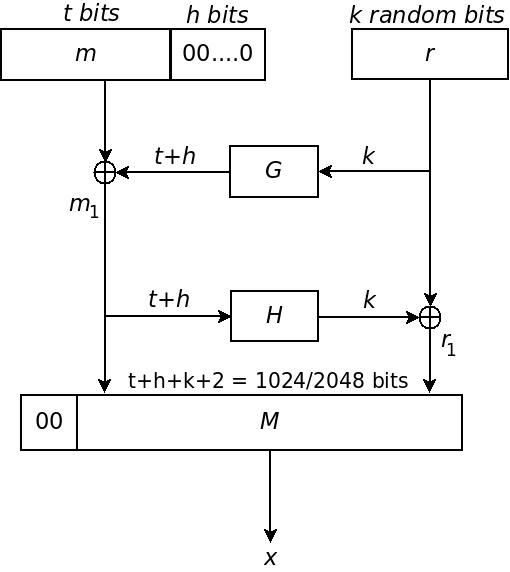
\includegraphics[width=0.45\textwidth]{OAEP.jpg}
\end{center}
Consideriamo \textit{n} è il numero di bit nel modulo RSA, \textit{h} e \textit{k} sono costanti intere fissate dal protocollo ed \textit{m} è il messaggio in chiaro, ovvero una stringa lunga $n - k - h - 2$. Definiamo ora \textbf{\textit{G}} e \textbf{\textit{H}} come due funzioni di \textit{hash crittografico}. Andiamo ad analizzare i passaggi per cifrare:
\begin{enumerate}
    \item al messaggio \textit{m} va applicato un \textit{padding} di \textit{h} zeri per arrivare alla lunghezza di $n - k - 2$
    \item definiamo \textit{r} come una stringa casualmente generata di \textit{k} bit
    \item \textit{r} verrà poi espansa da \textit{k} a $n - k - 2$ bit tramite la funzione di hash \textbf{\textit{G}}
    \item $m_1 = m \oplus G(r)$
    \item tramite \textbf{\textit{H}} $m_1$ viene ridotta da $n - k - 2$ bit a \textit{k} bit.
    \item $r_1 = r \oplus H(m_1)$
    \item il messaggio finale, che verrà successivamente convertito in un numero \textit{x} da mandare come input ad RSA è ``$00\;||\;m_1\;||\;r_1$''
\end{enumerate}
La \textbf{decifrazione} è definita dalle proprietà dello \textbf{\textit{xor}} logico.

\newpage
\section{Sistema Crittografico Asimmetrico di Rabin}
Poco dopo l'introduzione di \textit{RSA}, \textbf{Michael O. Rabin} ha sviluppato un algoritmo crittografico a cui appartiene la proprietà teorica di essere equivalente alla fattorizzazione, ovvero un algoritmo \textit{polynomial time} in grado di violare il sistema di \textit{Rabin} potrebbe essere utilizzato per la fattorizzazione di interi (e viceversa), ma, come contro, presenta una limitazione in quanto la decifrazione di un ciphertext arbitrario produce \textbf{quattro possibili} candidati come \textbf{plaintext}. Andiamo ad analizzare le quattro possibili radici di un numero $y \in \mathbb{Z}_p^*$ attraverso un esempio numerico.
\begin{center}
    Definiamo: $p = 13 \;\; q = 23 \;\; n = p \cdot q = 299$ \\
    Prendiamo un elemento $x \in \mathbb{Z}_p^*$: $x = 27$ \\
    Calcoliamo il suo quadrato: $ y = x^2 \bmod n = 131$ \\  
    Sappiamo che in $\mathbb{R} \Rightarrow \sqrt{131} = \pm x$ \\
    Allora anche in $\mathbb{Z}_n^*$ saranno presenti due radici: $(x, -x)$ \\
    Calcoliamo $-x = n - x = 272 \Rightarrow (-x)^2 \bmod n = 131$ \\
    Precalcoliamo $c_p = q \cdot (q^{-1} \bmod p) = 92 \;\;\; c_q = p \cdot (p^{-1} \bmod q) = 208$
\end{center}
Consideriamo ora che $n = p \cdot q$ utilizzando il \textit{CRT} sappiamo che data l'equazione $\exists \: C \; | \; C \equiv y \bmod n, \; C = c_p * a_1 + c_q * a_2$, prima di tutto andiamo a calcolarci le quantità $a_1 \text{ e } a_2$, come $a_i = y \bmod n_i, \;\; i = \{p, q\}$, $a_1$ è il corrispondente di \textit{y} in $\mathbb{Z}_p^*$ e, ovviamente $a_2$ è il corrispondente di \textit{y} in $\mathbb{Z}_q^*$. Allora sia per $a_1 \text{ che per } a_2$ saranno presenti 2 radici, rispettivamente in $\mathbb{Z}_p^*$ e in $\mathbb{Z}_q^*$, possiamo calcolarli come:
\begin{center}
    $x_{p^1} = y^{(2^{-1} \bmod p)} \bmod p = 1$ \\
    $-x_{p^1} = x_{p^2} = p - x_{p^1} = 12$ \\
    $x_{q^1} = y^{(2^{-1} \bmod q)} \bmod q = 4$ \\
    $-x_{q^1} = x_{q^2} = q - x_{q^1} = 19$ \\
    Per trovare le radici di \textit{y} in $\mathbb{Z}_n^*$ applicando il \textbf{\textit{CRT}} avremo: \\
    $x_1 = c_p * x_{p^1} + c_q * x_{q^1} = 27$ \\
    $x_2 = c_p * x_{p^1} + c_q * x_{q^2} = 157$ \\
    $x_3 = c_p * x_{p^2} + c_q * x_{q^1} = 142$ \\
    $x_4 = c_p * x_{p^2} + c_q * x_{q^2} = 272$ \\
\end{center}
Alla fine avremo che $y = x_i^2 \bmod n = 131\;\; \forall i = 1, 2, 3, 4$, siamo riusciti a ``dimostrare'' che preso un \textit{quadrato perfetto} in $\mathbb{Z}_n*$ con \textit{n} che è il prodotto di due numeri \textit{coprimi} tra loro, il quadrato perfetto avrà quattro \textbf{radici} in $\mathbb{Z}_n*$, due delle quali saranno fra loro \textbf{congrue modulo p} e due \textbf{congure modulo q}. Riuscendole ad ottenere applicando il \textit{CRT}.
\\ \newline
Descriviamo ora l'\textbf{algorimo generale}, anche in questo caso verrà diviso in generazione delle chiavi, che necessita come input un solo parametro, ovvero la lunghezza in bit di \textit{n}. E una parte di scambio di informazioni che quindi necessiterà di utilizzare cifratura e decifratura.
\begin{itemize}
    \item \textbf{Generazione delle chiavi: \textit{Alice}}
    \begin{enumerate}
        \item genera due numeri primi a caso di lunghezza $\frac{n}{2}$ bit tale che $p \equiv 3 \bmod 4$ e $q \equiv 3 \bmod 4$.
        \item calcolo di $n = p \cdot q$.
        \item diffonde \textit{n} come \textbf{chiave pubblica} e conserva la coppia \textit{(p, q)} come \textbf{chiave segreta}.
    \end{enumerate}
    \item \textbf{Cifratura di un messaggio: \textit{Bob}}
    \begin{enumerate}
        \item si procura la chiave pubblica \textit{n} di \textit{Alice}.
        \item calcola $C = M^2 \bmod n$.
        \item invia \textit{C} ad \textit{Alice} come messaggio cifrato.
    \end{enumerate}
    \item \textbf{Decifrazione del messaggio \textit{C}: \textit{Alice}}
    \begin{enumerate}
        \item \textit{Alice} calcola $M_p = C^{\frac{p + 1}{4}} \bmod p$ e $M_q = C^{\frac{q + 1}{4}} \bmod q$, notiamo che $M_p$ è una delle \textit{radici quadrate di C} modulo \textit{p} perché:
        \begin{center}
            \begin{math}
                \begin{aligned}
                    M_p^2 \bmod p &= (C^{\frac{p + 1}{4}})^2 \bmod p \\
                    &= C^{\frac{p + 1}{2}} \bmod p \\
                    &= C^{\frac{p - 1}{2}} \cdot C \bmod p \\
                    &= ((M^2 \bmod n)^{\frac{p - 1}{2}} \cdot C) \bmod p \\
                    &= (((M^2 \bmod n) \bmod p)^{\frac{p - 1}{2}} \cdot C) \bmod p \\
                    &= ((M^2 \bmod p)^{\frac{p - 1}{2}} \cdot C) \bmod p \\
                    &= (M^{p - 1} \cdot C) \bmod p \\
                    &= (1 \cdot C) \bmod p \\
                    &= C \bmod p
                \end{aligned}
            \end{math}
        \end{center}
        Analogamente $M_p$ è una delle \textit{radici quadrate di C} modulo \textit{q}.
        \item riprendendo il discorso del \textit{CRT} possiamo calcolare le quattro radici di $C$ modulo \textit{n} e una di questi valori sarà il messaggio originale.
        \begin{center}
            $M_1 = ((q \cdot (q^{-1} \bmod p)) * M_p) + (p \cdot (p^{-1} \bmod q) * M_q) \bmod n = (c_p \cdot M_p + c_q \cdot M_q) \bmod n$ \\
            $M_2 = n - M_1 = ((-c_p) \cdot M_p + (-c_q) \cdot M_q) \bmod n$ \\
            $M_3 = ((q \cdot (q^{-1} \bmod p)) * M_p) - (p \cdot (p^{-1} \bmod q) * M_q) \bmod n = (c_p \cdot M_p + (-c_q) \cdot M_q)$ \\
            $M_4 = n - M_3 = ((-c_p) \cdot M_p + c_q \cdot M_q) \bmod n$ 
        \end{center}
        Utilizzando il \textit{CRT} possiamo verificare che, effettivamente, \textit{M} è effettivamente una delle quattro radici di \textit{C} modulo \textit{n}.
    \end{enumerate}
\end{itemize}
\   \\
\textbf{Equivalenza con il problema della fattorizzazione}
\newline
Dobbiamo dimostrare che se siamo in grado di decifrare (con un incertezza 1 su 4) allora possiamo fattorizzare \textit{n}, il viceversa è ovvio. Abbiamo visto che le quattro radici di $C \bmod n$ corrispondono alle quattro possibili combinazioni delle due radici modulo \textit{p} e delle due radici modulo \textit{q}:
\begin{enumerate}
    \item $M_1$ corrisponde alla coppia $(M_p, M_q) = (C^{\frac{p + 1}{4}} \bmod p, C^{\frac{q + 1}{4}} \bmod q)$.
    \item $M_2$ corrisponde alla coppia $(p - M_p, q - M_q)$ .
    \item $M_3$ corrisponde alla coppia $(M_p, q - M_q)$.
    \item $M_4$ corrisponde alla coppia $(p - M_p, M_q)$.
\end{enumerate}
L'obiettivo è fattorizzare un numero \textit{n} dato in input e considerare di possedere una scatola \textbf{black-box} che contenga l'algoritmo di dato un numero \textit{C}, resido quadratico in modulo \textit{n}, restituirti una delle quattro radici. \\
La riduzione è un algoritmo tipo \textbf{Las Vegas} e funziona in questo modo:
\begin{enumerate}
    \item genero a caso un numero $r \in \mathbb{Z}_n, r \neq 0$.
    \item se $m = gcd(r, n) \neq 1$ restituisco \textit{m} e \textit{n/m}.
    \item altrimenti considero \textit{r} come un ``messaggio'', calcolo $C = r^2 \bmod n$ e sottopongo \textit{C} alla black box.
    \item se $r'$ è il valore restituito dalla black-box, calcolo $m = gcd(r - r', n)$.
    \item se $m > 1 \text{ e } m \neq n$ restituisco i fattori \textit{m} e \textit{n/m}, altrimenti ritorno al passo \textit{1}.
\end{enumerate}
La correttezza è che la \textit{black-box} ritorna $r'$ che è una delle quattro radici di $C = r^2 \bmod n$ e che può essere uno dei quattro modi che abbiamo per combinare le due radici di $r^2 \bmod p$ e le due radici di $r^2 \bmod q$. Consideriamo che $r = (r_p, r_q) = (M_p, M_q)$ (esempio senza perdere di generalità).
\begin{enumerate}
    \item $r' = (r_p, r_q) = r$ allora avremo che $r - r' = 0$ ovvero che seguendo il \textit{CRT} avremo che $(r - r') \bmod p = r_p - (p - r_p) \bmod p = 2r_p \bmod p$ e che $(r -r') \bmod q = r_q - (q - r_q) \bmod q = 2r_q \bmod q$ e che quindi $n = m$ e che quindi non riusciamo a ad ottenere una risposta dall'algoritmo.
    \item $r' = (-r_p, -r_q) = -r$ allora avremo che $r - r' = 2r$ e quindi otteniamo $gcd(r, n) = 1$ e anche qui non riusciamo a determinare i fattori di \textit{n}.
    \item $r' = (r_p, - r_q)$ allora avremo che $r - r' = (r_p, r_q) - (r_p, - r_q) = (r_p - r_p, r_q - (- r_q)) = (0, 2r_q)$ ma avere il fatto in modulo p a \textit{0} implica che nel \textit{CRT} il suo fattore modulo p sia $r_p = C^{\frac{p + 1}{4}} \bmod p = 0$ che implica che $C^{\frac{p + 1}{4}}$ sia multiplo con \textit{p} e quindi avremo che $gcd(r', n) = p$.
    \item $r = (-r_p, r_q)$ in questo caso avremo l'esatto opposto del punto precedente, ovvero che $r - r' = (2r_p, 0)$ in questo caso avremo che quindi nel fattore $r_p = C^{\frac{q + 1}{4}} \bmod q = 0$ del \textit{CRT} avremo che $C^{\frac{q + 1}{4}}$ sia multiplo con \textit{q} e quindi avremo che $gcd(r', n) = q$.
\end{enumerate}
\   \\
\textbf{Riduzioni Polinomiali} \\
Per riuscire a dimostrare che un algoritmo è ``uguale'' ad un altro, in questo caso dobbiamo dimostrare che l'\textbf{algoritmo di fattorizzazione} è ``uguale'' all'\textbf{algoritmo per la risoluzione di Rabin}, bisogna dimostrare che l'uno e l'altro abbiano uguale \textbf{complessità}. Nel caso di dimostrare che saper risolvere \textbf{Rabin} equivale a saper \textbf{FATTORIZZARE} è immediato infatti se sappiamo fattorizzare un  numero \textit{n} allora otteniamo \textit{p} e \textit{q} e quindi abbiamo la chiave privata di \textit{Alice}. Per dimostrare, invece, che risolvere \textbf{Rabin} vuol dire risolvere il problema della \textbf{FATTORIZZAZIONE} abbiamo utilizzato il sistema della \textbf{black box}, ovviamente affinché questo funzioni la \textit{black box} deve ritornare una della quattro radici in maniera casuale.